\documentclass[10pt]{article}
\usepackage{mymacros}

\mytitle{Matrix Pencil Sparse Fourier Transform}
\myauthor{Jiawei Chiu, Laurent Demanet}
\mydate

\begin{document}
\pagestyle{plain}
\maketitle

\section*{Disclaimer}
This is not a formal publication. We try to be brief.

\section{Introduction}
Given a $N$-vector $x$, we like to perform the forward FFT to obtain $\hat{x}$. This is typically done in $O(N \log N)$ time. However, suppose we know that $\hat{x}$ is $S$-sparse plus some noise. Then it is possible to recover these $S$ modes in $\tilde{O}(S)$ time where $\tilde{O}(\cdot)$ is $O(\cdot)$ notation ignoring log factors. We call such algorithms SFT algorithms.

SFT is not new. Existing work includes AAFFT\cite{iwen2007empirical}, sFFT3.0\cite{hassanieh2012simple, hassanieh2012nearly}. However, these algorithms have seen little use because $n$ has to be very large relative to $S$ in order to justify its use.

In a study done by creators of sFFT3.0, where noiseless inputs are assumed, AAFFT is faster than FFTW\cite{FFTW05} only when $k\lesssim 2^8$. In our benchmarks, MPSFT, our new SFT algorithm, is faster than FFTW when $k \lesssim 1800$, when we consider rather noisy inputs. We believe there is \textbf{at least a 5X improvement} over AAFFT. Note that we do not consider sFFT3.0 because it works only for noiseless inputs.

Before proceeding, we set up some notation. We use the following convention:
$$x_t = \sum_k \hat{x}_k e^{2\pi i kt/N}; \quad \hat{x}_k =\frac{1}{n} \sum_t x_t e^{-2\pi i k t/N}.$$

In the noiseless case, the support of $\hat{x}$ are integers and we call them \textbf{mode locations}. When these are divided by $n$ and mapped into $[0,1)$, we call them \textbf{mode frequencies}. We use these interchangeably.

There are three new ingredients in MPSFT:

\begin{enumerate}
\item \textbf{Matrix pencil method}: The matrix pencil method, like the Prony method, is a standard technique in signal processing for mode frequency identification.

In this work, we integrate the matrix pencil method into the SFT framework to achieve two effects. Firstly, it identifies modes much more accurately than what is used in existing SFT algorithms. Secondly, it helps detect errors in our mode identification step and greatly reduces the number of spurious modes being found. In existing SFT algorithms, we pay a much heavier cost to filter away or undo such modes.

\item \textbf{Exploiting symmetry}: Matrix pencil method is more accurate for mode identification, but it comes at a cost. The straightforward way of using it would double the time needed for mode identification. We realize that this cost can be roughly halved if we exploit some symmetry in the matrix pencil method.

\item \textbf{SIMD vectorization}: FFTW makes good use of SIMD instructions. To be competitive, we vectorize critical parts of our code using OMP-SIMD and Boost-SIMD. This yields at least a 2X improvement in running time.

\end{enumerate}

\section{SFT framework}

Before we can discuss MPSFT, we need to describe the typical SFT framework, from our perspective. We begin with a summary.
\begin{itemize}
\item SFT algorithms are \textbf{iterative}. We aim to find a constant proportion of nodes in each iteration.

\item \textbf{Bin} these modes and obtain $B$ bin coefficients. Each bin coefficent $U_b$ is a sum over roughly $N/B$ mode locations:
$$U^b \simeq \sum_k \hat{x}_k \hat{W}_{b,k} \text{ where } \hat{W}_{b,k} \simeq \text{Indicator}(\lfloor kB/N \rfloor = b).$$

\item Binning can be done in $\tilde{O}(B)$ time on $x$ instead of $\hat{x}$ using signal processing tricks.

\item SFT algorithms are \textbf{probabilistic}. Choose number of bins $B$ to scale with $S$ such that when modes are randomly permuted, there is a decent chance that some bins contain exactly one mode. We call this \textbf{mode isolation}.

\item If bin $b$ has an isolated mode $k_*$, then $U^b \simeq \hat{x}_{k_*}$. This yields the mode coefficient but not the mode location yet.

\item Consider binning being applied to $\hat{x}$ modulated by $\tau$ (which corresponds to $x$ being translated by $\tau$). For each $\tau$, we have $B$ bin coefficients:
$$U^b_{\tau} \simeq \sum_k \hat{x}_k \hat{W}_{b,k} e^{2\pi i k \tau/N}.$$

\item \textbf{Small but important observation}: $U^b_{\tau}$ can be viewed as a signal sampled at location $\tau$. We call $U^b$ a \textbf{binned signal}.

\item When there is mode isolation in bin $b$, then $U^b$ is a signal with only one mode and we can identify this mode using techniques such as the matrix pencil method.

\item As an example, sFFT3.0 samples $U^b$ at only two points $\tau=0,1$. When there is mode isolation in bin $b$, then
$$U^b_1/U^b_0 \simeq e^{2\pi i k_*\tau/N}.$$
It is clear that its argument or angle yields $k_*$, the mode location we want.

\item This can only tolerate an error of $O(1/N)$ in the frequency estimation, which does not work in the noisy case.

\item In the noisy case, we \textbf{dilate in frequency space} by powers of $2$ in order to discover each \textbf{bit} of the mode frequency. Each bit can tolerate $O(1)$ error.

\item For each bit, we can also do multiple independent measurements and use \textbf{probability amplification} to further drive down the chance of getting the bit wrong.

\end{itemize}

Now, we provide more details.

\subsection{Random transformation for mode isolation and denoising}
Let $y$ be the transformed signal. It is transformed using three parameters $a,b,c$. Modes are permuted according to $a, b$ and modulated according to $c$:
$$\hat{y}_{\phi(k)} = \hat{x}_k e^{2\pi i ck/N}$$
where $\phi(k) = ak+b$. Correspondingly, in time space, we have
$$y_t = x_{at+c} e^{2\pi i bt/N}.$$

The mode permutation $(a,b)$ is to achieve mode isolation.

The mode modulation $c$ is to make the noise incoherent. It is a denoising mechanism. The basic idea is this. Say there is mode isolation. For simplicity, say there is only one bin and $W_{b,k}=1$. Then
$$U^b_0 = \hat{x}_{k_*}e^{2\pi i c k_*/N} + \sum_{k\neq k_*} \hat{x}_k e^{2\pi i c k/N}.$$
The error term can be written as
$$U^b_0 e^{-2\pi i c k_*/N} -\hat{x}_{k_*} = \sum_{k\neq k_*} \hat{x}_k e^{2\pi i c(k-k_*)/N}.$$

Take expectation over the random $c$. Clearly the LHS has zero mean and its variance is $\sum_{k\neq k_*} |\hat{x}_k|^2$. We call this the \textbf{noise energy}. With a random $c$, we limit the distortion of our bin coefficients from $\sum_{k\neq k_*} |\hat{x}_k|$ (coherent noise) to $\sqrt{\sum_{k\neq k_*} |\hat{x}_k|^2}$.

\subsection{Binning in time domain}

Say we want to bin a signal $y$. Let $B$ be number of bins. The basic idea is we want to convolve with a boxcar filter in the frequency domain. But the boxcar filter is the sinc function which decays slowly in the time domain. Binning, if executed from the time domain, would require sampling $N$ points. To get around that, we smooth or convolve the boxcar filter with the Gaussian. In the time domain, this means our filter is multiplied by a Gaussian. It decays rapidly and can be truncated to have a support of $\tilde{O}(B)$.

Let $\delta>0$ be a small value controlling the accuracy of our window. Let $c_{\delta} = \log (1/\delta)$. Let $\sigma_f = \frac{1}{4B\sqrt{2c_{\delta}}}$ and $\sigma_t = \frac{1}{2\pi \sigma_f}$. Let $w=\frac{1}{2B}$ be the desired halfwidth of the window in frequency space. In the time domain, we want to first \textbf{multiply} our input signal with $e^{-2\pi i t/2B}W_t$ where the window function is 
$$W_t = e^{-t^2/2\sigma_t^2} F_{w,t} \text{Indicator}\left(|t|\leq \frac{P-1}{2}\right)$$
where $F_{w,t} = \frac{\sin(\pi t w)}{\pi t}$ is the sinc function, and $P$ decides the support of our window, and is an odd integer satisfying $P \geq 2\sigma_t \sqrt{2c_{\delta}} + 1$. This first step takes $O(P)=O(B c_{\delta})$ time. (Do not worry about the $e^{-2\pi i t/2B}$ term. It is just to shift by $0.5/B$ in the frequency space so that bin edges are $0, 1/B, 2/B, \ldots$ instead of $0.5/B, 1.5/B, 2.5/B, \ldots$.)

The second step is to \textbf{fold} our $P$ vector into a $B$-vector, which corresponds to subsampling the convolution of $\hat{x}$ with our boxcar filter, at $B$ points. Recall Poisson summation formula if interested.

The third step is to perform a $B$-point \textbf{dense FFT} on our folded vector. This takes $O(B\log B)$ time. We can use FFTW for this step.

In practice, almost all of the time is taken up by the first step, because of the many expensive trignometric function evaluations.

\subsection{Binning in frequency domain}

SFT is an iterative algorithm. As modes are found, they have to be implicitly removed from the original input signal. This means when we bin a signal, we need to \textbf{subtract contributions} to bin coeffcients due to found modes.

Binning in frequency domain is much easier than binning in time. Say our input signal is $y$. For each mode $k_*$ in the input signal, we first find the bin it is in by $b = \lfloor k_* B/N \rfloor$. Then multiply $\hat{y}_{k_*}$ by
$$\hat{W}_{b,k_*} = \hat{W}\left(\frac{b+0.5}{B}-\frac{k_*}{N}\right)$$
where
$$\hat{W}(\xi)=\frac{1}{\sigma_f \sqrt{2\pi}} \int_{\xi-1/4B}^{\xi+1/4B} e^{-\eta^2/2\sigma_f^2} d\eta.$$

Finally, subtract $\hat{y}_{k_*} \hat{W}_{b,k_*}$ from the $b$-th bin coefficient.

Note that the input argument to $\hat{W}(\xi)$ is the offset of $k_*/N$ from the bin center $\frac{b+0.5}{B}$ in frequency space $[0,1)$.  Note that the integral can be evaluated fast using \texttt{erf}. Note that $\hat{W}(\xi)$ is not exactly the Fourier transform of $W_t$. In the frequency domain, $\hat{W}(\xi)$ would be off by $O(\delta)$. We are not going into this error analysis here, but may add an appendix later.

\subsection{Binning can denoise}

Earlier in the section on random transformation, we saw that bin coefficients are distorted by $\sim \sqrt{\sum_{k\neq k_*} |\hat{x}_k|^2}$ or the square root of the noise energy.

If you repeat the analysis for more than one bin, the variance of the error in each bin coefficient works out to be $\sum_{k\neq k_*} |\hat{x}_k \hat{W}_{b,k}|^2$.

Let $\Lambda$ be the set of heavy modes. Define the overall noise energy to be $\sigma^2 := \sum_{k\neq \Lambda} |\hat{x}_k|^2$. Then the above formula suggests that the error in each bin coefficient would be usually be on the order of $\frac{\sigma}{\sqrt{B}}$. Even in later iterations when $S$ of the residual signal is very small, we still want to maintain a \textbf{minimum number of bins} to mitigate the error in bin coefficients by $1/\sqrt{B}$. This is essential for ensuring a good chance of mode identification.

\subsection{Translating by $\tau$}

Denote $x$ as the original signal and $y$ as the transformed signal using parameters $a,b,c$.

In the summary, we mention that we want to bin not just $y$, but also $y$ modulated in the frequency space for the purpose of \textbf{mode identification}. Denote $y^{\tau}$ as $y$ modulated by $\tau$ in frequency domain, that is
$$y^{\tau}_{t} = y_{t+\tau}; \quad \hat{y}^{\tau}_k = \hat{y}_k e^{2\pi i k \tau/N}.$$

To recap, we have the following signals:
$$x \xrightarrow{a,b,c} y \xrightarrow{\tau} y^{\tau}.$$

Note that binning is applied to each $y^{\tau}$ signal. Binning takes up almost all the running time of SFT algorithms. Hence, each additional $\tau$ we add comes at great cost. sFFT3.0 only needs $\tau=0,1$ because it assumes no noise. It is not surprisingly that it is so fast. However, in the noisy case, as we see in the next section, we need many more $\tau$'s.

\subsection{Mode identification}

Mode identification is applied to the \textbf{binned signal} $U^b$ for each bin $b$. For all discussion related to mode identification, we fix a bin $b$ and let $U=U^b$ to avoid writing the $b$ superscript.

Say our input signal is $U_{\tau} \simeq \hat{y}_{k_*} e^{2\pi i k_* \tau/N}$. As we saw in sFFT3.0, $U_1/U_0 \simeq e^{2\pi i k_* \tau/N}$. Using this method, to recover $k_*$ \textbf{exactly}, we need to estimate the frequency $k_*/N$ within $O(1/N)$ accuracy. In other words, $U_1/U_0$ cannot be perturbed by no more than $O(1/N)$. That means the error in each bin coefficient $U_0^b,U_1^b$ has to be $O(|\hat{W}_{b,k_*}\hat{y}_{k_*}|/N)$.

For simplicity, we assume that all heavy modes has at least magnitude $1$ and we reject modes when $\hat{W}_{b,k_*}$ is below a fixed threshold. Hence, the error in each bin coefficient has to be $O(1/N)$. Since this error decreases with $1/\sqrt{B}$, we would need $B=\Omega(N^2)$, which would make SFT algorithms slower than dense FFT algorithms!

Instead of trying to estimate $k_*/N$ within $O(1/N)$ accuracy, we shall \textbf{estimate which half $k_*/N$ is in} or the first bit of $k_*/N$. This would succeed as long as the error in the bin coefficient is roughly smaller than the distance of $k_*/N$ from the decision edges $0, 0.5$. Another way to put it is that $k_*/N$ is some distance away from $0, 0.5$ and its perturbation does not move it from one half to another.

Due to the random permutation, there is a good chance that $k_*/N$ is $\Omega(1)$ away from these $0,0.5$ edges, so we can tolerate a $O(1)$ error in the bin coefficients. This means $B$ has to be $\Omega(1)$ instead of the previous nonsensical $\Omega(N^2)$.

After getting the first bit of $k_*/N$, we try to get the second bit by dilating $U_{\tau}$ in the frequency space. Specifically, for $s\geq 0$, consider $\tau=0,2^s$ and compute
$$U_{2^s}/U_0 \simeq e^{2\pi i k_* 2^s/N}.$$
Seeing which half of the complex plane $U_{2^2}/U_0$ is in tells us the $s$-th bit of $k_*/N$. Repeat this $\sim \log_2 N$ times to recover $k_*/N$ up to $O(1/N)$ accuracy.

Two more tweaks and we have the basic framework for mode identification.

The first tweak is that since $k_*$ is in some bin $b$, there are only $N/B$ possibilities not $N$. Thus, we only need to estimate $\sim \log_2 (N/B)$ bits not $\log_2 N$, and the $\tau$'s used would be $0, B, 2B, 2^2 B, 2^3 B, 2^4 B, \ldots$. In other words, we further dilate $y$ by a factor of $B$ in frequency space.

The second tweak has to do with \textbf{probability amplification}. For example, instead of only doing $U_{1}/U_0$, we can do $U_{q+1}/U_q$ for multiple different random $q$'s, and use \textbf{majority voting} to decide which half $k_*/N$ is in. The probability of identifying this bit wrongly would decrease exponentially with the number of different $q$'s used.

Suppose we obtain a $m$-bit integer $z$. Then we can estimate the frequency $k_*/N$ as $\frac{z+0.5}{2^m} \frac{1}{B} + \frac{b}{B}$. Multiply this by $N$ and round off to estimate $k_*$. In other words, estimate $k_*$ as
$$\text{round}\left( \frac{N}{B} \left( \frac{2z+1}{2^{m+1}} + b\right)\right).$$

\section{MPSFT enhancements}

We are now ready to discuss our enhancements of the typical SFT algorithm in the previous section.

\subsection{Matrix pencil method}
We will not discuss the full matrix pencil method. Fix a bin $b$ and consider the binned signal $U=U^b$. We consider only the case where we sample the input signal $U$ at three points $-1, 0, +1$. Form the matrix
$$M = \frac{1}{2} \left( \begin{array}{cc}
U_0 & U_{-1} \\
U_{1} & U_0
\end{array} \right).$$

Compute the \textbf{SVD} of this $2\times 2$ matrix. If the second singular value is sufficiently large, say $\Omega(\sigma/\sqrt{B})$, then there is probably a \textbf{mode collision}, i.e., no mode isolation in this bin. Note that $\sigma^2$ is the overall noise energy and $\sigma^2= \sum_{k\neq \Lambda} |\hat{x}_k|^2$ where $\Lambda$ is the set of heavy modes.

In existing SFT algorithms, there are various ways of handling wrongly identified modes. One way is to sort all the found modes by their magnitude in each iteration, and drop the smallest ones. Another way is to use larger $B$ and more conservative parameters to make sure that these wrong modes would be corrected in subsequent iterations. These are all much more expensive compared to this cheap SVD step.

Furthermore, this SVD step \textbf{denoises the binned signal} $U$ as we consider only the dominant singular vector. Let $v$ be the dominant right singular vector. Then $$\text{imag}(\text{conj}(v_0)v_1)<0$$ is a vote for the isolated frequency being in the second half $[0.5,1)$ of the frequency space, i.e., the first bit of $k_*/N$. In a \href{https://github.com/tinkerstash/mpsft/blob/master/notebook/Mode%20identification.ipynb}{simple numerical experiment}, it boosts the chance of getting this bit right from $70\%$ to $80\%$.

Above, we use $\tau=-1,0,1$ for simplicity. In MPSFT, we actually sample $U$ at $\tau=q \pm 2^s B$ for $s=0,\ldots,1 + \lfloor \log_2 (N/B) \rfloor$ and multiple random $q$'s. For each $(q-2^s B, q, q+2^s B)$, we have a vote for the $s$-th bit of $k_* B/N$. For each $s$, we sum the votes over different $q$'s and take the majority.

\subsection{Exploiting symmetry to halve number of trigonometric operations}

Fix a bin $b$. For simplicity, assume only one $q$ and for the matrix pencil method, we need to sample $U=U^b$ at $\tau=q, q\pm s$ for multiple different $s$'s. On the other hand, for the method of simple ratios where we consider which half $U_{q+s}/U_q$ is in, we only need to sample $U$ at $q, q+s$ for multiple different $s$'s. In other words, the matrix pencil method seems to demand twice as much work!

Fortunately, due to the \textbf{symmetry} in these $\tau$'s, we could halve the number of trignometric operations, which roughly \textbf{halves the cost of matrix pencil method}. The implication is that compared to the method of simple ratios, the matrix pencil method is hardly more expensive but offers advantages such as collision detection and denoising.

Recall we currently have the following schematic:
$$x \xrightarrow{a,b,c}{y} \xrightarrow{q,s} y^{q\pm s}.$$

Consider the following. Let $z=y^q$ such that $\hat{z}_k = \hat{y}_k e^{2\pi i k q/N}$. Derive $z^R, z^I$ from $z$ by taking real and imaginary components in frequency space:
$$\hat{z}^R_k=\text{Re}(\hat{z}_k); \quad \hat{z}^I_k = \text{Im}(\hat{z}_k); \quad \hat{z}_k = \hat{z}_k^R + i \hat{z}_k^I.$$
In the time domain, $z^R,z^I$ are even and odd components of $z$:
$$z^R_t = \frac{1}{2}(z_t + \text{conj}(z_{-t})); \quad z^I_t = \frac{1}{2i}(z_t - \text{conj}(z_{-t})); \quad z_t = z_t^R + i z_t^I.$$

Now, modulate $z^R, z^I$ in frequency domain, or translate $z^R,z^I$ in time domain to obtain $z^{R,s}, z^{I,s}$. Specifically,
$$z^{R,s}_{t}=z^R_{t+s}; \quad z^{I,s}_{t}=z^I_{t+s}$$
and
$$\hat{z}^{R,s}_{t}=\hat{z}^R_{k}e^{2\pi i s k/N}; \quad \hat{z}^{I,s}_{k}=\hat{z}^I_{k} e^{2\pi i sk/N}.$$

The new schematic is
$$x \xrightarrow{a,b,c}{y} \xrightarrow{q} z \rightarrow z^R, z^I \xrightarrow{s} z^{R,s}, z^{I,s}.$$

Binning is applied to $z^{R,s}, z^{I,s}$ to obtain binned signal $V^R, V^I$ (associated with $z^R, z^I$ respectively) sampled at $s$:
$$V^{R}_s = \sum_k \text{Re}(\hat{z}_k) \hat{W}_{b,k} e^{2\pi i ks/N};\quad V^{I}_s = \sum_k \text{Im}(\hat{z}_k) \hat{W}_{b,k} e^{2\pi i ks/N}.$$

Observe that once $V^R_s,V^I_s$ are computed, they can be \textbf{recombined cheaply} to give us $U_{q\pm s}$:
$$U_{q+s} = V^{R}_s + i V^I_s; \quad U_{q-s} = \text{conj}(V^{R}_s) + i \text{conj}(V^{I}_s).$$
We have made use of the fact that $\text{conj}(\hat{W}_{b,k} e^{2\pi i ks/N}) = \hat{W}_{b,k} e^{-2\pi i ks/N}$.

Next, we see how to compute $V^R_s, V^I_{s}$ fast.

\subsubsection{Binning in frequency domain}

Previously, we need to compute one $e^{2\pi i \theta}$ term per $(k, \tau)$. Now, consider binning $z^{R,s},z^{I,s}$.

The bin coefficients we want are as follows.
$$V^R_s = \sum_k \text{Re}(\hat{y}_k e^{2\pi i qk/N}) \hat{W}_{b,k} e^{2\pi i k s/N} = \sum_k \text{Re}(\hat{x}_k e^{2\pi i ck/N} e^{2\pi i q \phi(k)/N})\hat{W}_{b,\phi(k)} e^{2\pi i \phi(k) s/N}.$$
We also want
$$V^I_s = \sum_k \text{Im}(\hat{x}_k e^{2\pi i ck/N} e^{2\pi i q \phi(k)/N})\hat{W}_{b,\phi(k)} e^{2\pi i \phi(k) s/N}.$$

Our outer loop is over found modes and the inner loop is over different $s$'s. Per found mode $k$, we compute $e^{2\pi i ck/N} e^{2\pi i q \phi(k)/N}$ only once as it does not depend on $s$. In the inner loop over $s$'s, we need to compute only one $e^{2\pi i \theta}$ term $e^{2\pi i \phi(k)s/N}$ and it is used for both $V^R_s$ and $V^I_s$.


\subsubsection{Binning in time domain}
For binning $z^{R,s}$ in time domain, we need to evaluate the following at $P$ different $t$'s:
$$\frac{1}{2} ( z_{t+s} + \text{conj}(z_{-(t+s)})) e^{-2\pi i t/2B} W_t$$
which is
$$\frac{1}{2}(y_{q+t+s} + \text{conj}(y_{q-(t+s)})) e^{-2\pi i t/2B}W_t$$
which is
$$\frac{1}{2}\left(x_{a(q+t+s)+c}e^{2\pi i b(q+t+s)/N} + \text{conj}(x_{a(q-(t+s))+c} e^{2\pi i b(q-(t+s))/N})\right) e^{-2\pi i t/2B}W_t$$
which can be factored as
$$\frac{1}{2} \left( x_{a(q+t+s)+c} A + \text{conj}(x_{a(q-(t+s))+c} A)\right)e^{2\pi i ((t+s)/N - 1/2B)} W_t $$
where $A:= e^{2\pi i bq/N}$ does not depend on $s, t$. Observe that per $(s, t)$, the most expensive operation is computing one single $e^{2\pi i ((t+s)/N - 1/2B)}$.

Now, consider binning $z^I$ in time domain. We need to compute
$$\frac{1}{2i} ( z_{t+s} - \text{conj}(z_{-(t+s)})) e^{-2\pi i t/2B} W_t$$
which will work out to be
$$\frac{1}{2i} \left( x_{a(q+t+s)+c} A - \text{conj}(x_{a(q-(t+s))+c} A)\right)e^{2\pi i ((t+s)/N - 1/2B)} W_t.$$

Observe that we can \textbf{reuse} the $e^{2\pi i ((t+s)/N - 1/2B)}$ term used for binning $z^R$.

To summarize, to bin $z^{R,s}, z^{I,s}$ in time domain, we need to evaluate only roughly $P m$ terms of the form $e^{2\pi i \theta}$ where $m$ is the number of different $s$'s. Doing it directly would have required roughly $2P m$ such terms.

\subsection{SIMD vectorization}

Our CPU is a I7-6700K which supports AVX2 but not AVX512. AVX2 has integer intrinsics, but only for int32 or smaller integers. Substantial amount of time is spent in computing $a(q+t+s)+c$ modulo $N$, but this has to be done in int64 and cannot be vectorized.

What can be vectorized is the sines and cosines involved in computing $e^{2\pi i \theta}$. Autovectorization with gcc using sin and cos in standard lib does not seem to work. We tried using our own Chebyshev approximation to achieve vectorization. However, the error incurred seems too much or some corner cases are not handled properly, which lead to convergence issues.

We eventually settle on using \textbf{Boost.SIMD}'s \cite{Esterie:2014:BGP:2568058.2568063} implementation of sincos. It runs as fast as our vectorized Chebyshev approximation, but provides much better accuracy. The convergence issues go away as a result.

\section{Benchmarks}

We assume the following input model for testing MPSFT. Let $N$ be a \textbf{prime} close to a power of $2$. Randomly generate $S$ mode locations. They are uniformly chosen from $[N]=\{0,1,\ldots,N-1\}$. Randomly generate $S$ mode coefficients each of \textbf{unit norm}. Basically, the coefficient's real and imaginary components are independent random Gaussians, and then it is normalized.

Next, we generate random noise in frequency domain. Let $\Lambda$ be the set of heavy modes generated earlier. We generate random Gaussians in $[N]-\Lambda$ and then normalize such that the \textbf{noise energy} is $\sigma^2$:
$$\sum_{k\neq \Lambda} |\hat{x}_k|^2 = \sigma^2$$
where $\sigma$ is user-provided. By the way, this means that in the time domain, each measurement is perturbed by a Gaussian with variance $\sigma^2$.

\subsection{Setup details}
Our CPU is a I7-6700K 4GHz. We disable CPU scaling and run Google Benchmarks with the flags \texttt{--benchmark\_repetitions=10} to obtain confidence intervals.

FFTW-3.3.6-pl2 is compiled locally with all the optimization turned on, for example \texttt{-O3} \texttt{-mtune-native} \texttt{-ffast-math}. We also run FFTW with $N$ being powers of $2$ only.

MPSFT is also compiled locally with \texttt{-O3} \texttt{-mtune=native} \texttt{-ffast-math} \texttt{-fopenmp-simd}. Note that we are using only OpenMP SIMD, and the program is \textbf{single-threaded}.

\subsection{Experiment: Fix $N$, vary $S$}
When $N$ is fixed, we want to know how small $S$ has to be for MPSFT to be competitive with FFTW.

Pick $N=4194301\simeq 2^{22}$. Fix the amount of noise by setting $\sigma=0.1$.

The $\delta$ controlling the accuracy of our window function is $10^{-5}$. Modes are rejected when $\hat{W}_{b,k}$ is below the threshold of $0.1$.

In each iteration, we set the number of bins $B$ to be $2S+1$ where $S$ is the total number of heavy modes minus the number of found modes. Fix the minimum of bins as $101$.

A bin is not processed if it does not have enough energy. This threshold is set as $\frac{3\sigma}{\sqrt{B}}$. A bin is also not processed if the second singular value reported by the matrix pencil method is too large. This threshold is set as $\frac{\sigma}{\sqrt{B}}$.

As the amount of noise is low, the number of trials used to identify each bit is set to $1$. However, even with only one trial, we can already tolerate much noise as we identify the mode frequency one bit at a time instead of trying to resolve it to $O(1/N)$ accuracy like in sFFT3.0.

MPSFT stops iterating when it hits a maximum number of stale iterations. An iteration is stale if no mode is found at all. This threshold is set as $5$ here.

We plot the results in Figure \ref{fig:runtime}. Errorbars are included and they are very small. For $N=2^{22}$, FFTW took around $0.242$ seconds. With some interpolation, we see that MPSFT is faster when $S\lesssim 1800$.


\begin{figure}
\centering
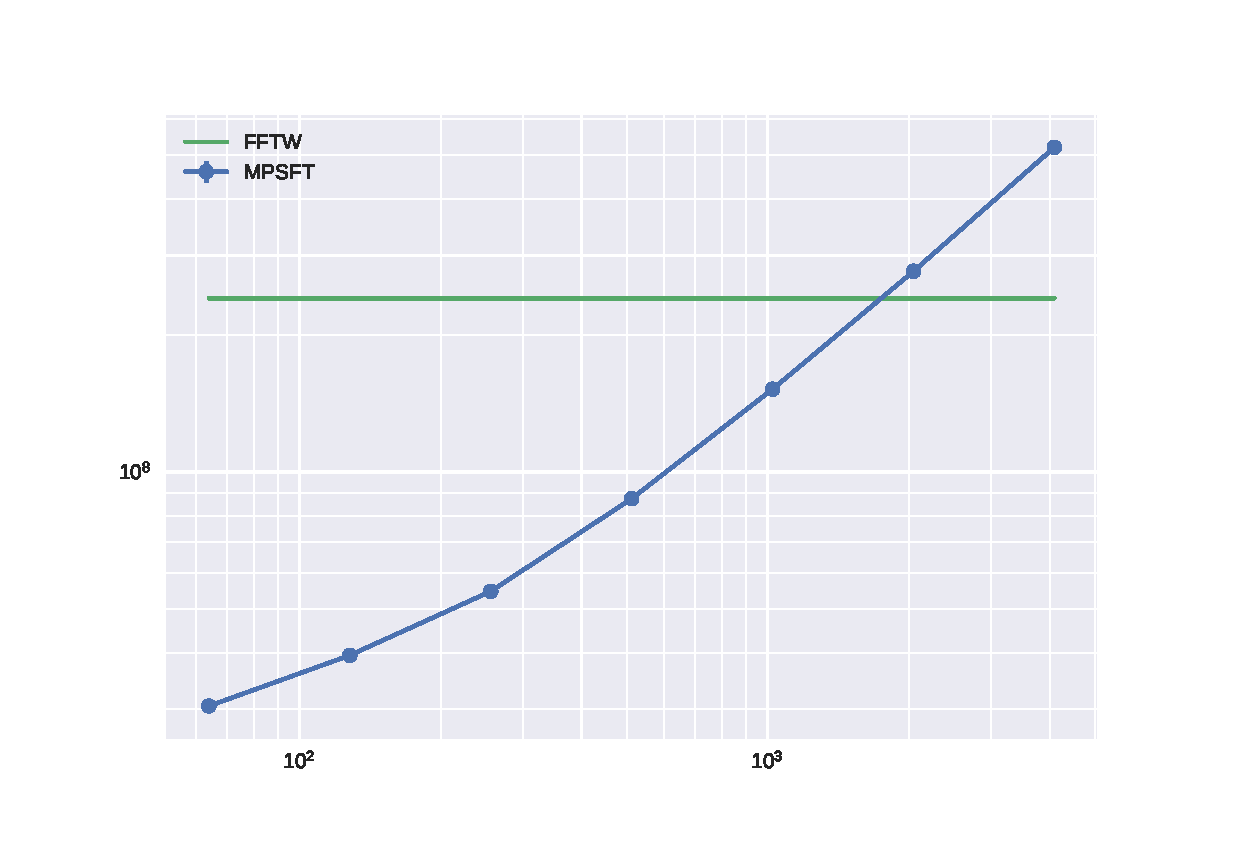
\includegraphics[scale=0.6]{./graph/runtime}
\caption{Loglog plot of running time versus sparsity $S$. The running time grows roughly linearly with $S$. Errorbars are very small. \label{fig:runtime}}
\end{figure}


\subsection{Experiment: Vary amount of noise}

Use the same parameters as the previous section. The only difference is that $\sigma$ is varied while $S$ is fixed at $1024$. Define the $L_1$ error or mean absolute error as $\frac{1}{N}\sum_k |\hat{x}_k - \hat{x}^{\text{est}}_k|$. We plot the mean $L_1$ error versus $\sigma$ on a log-log scale in Figure \ref{fig:noise}. Observe that this $L_1$ error decreases linearly with $\sigma$.

\begin{figure}
\centering
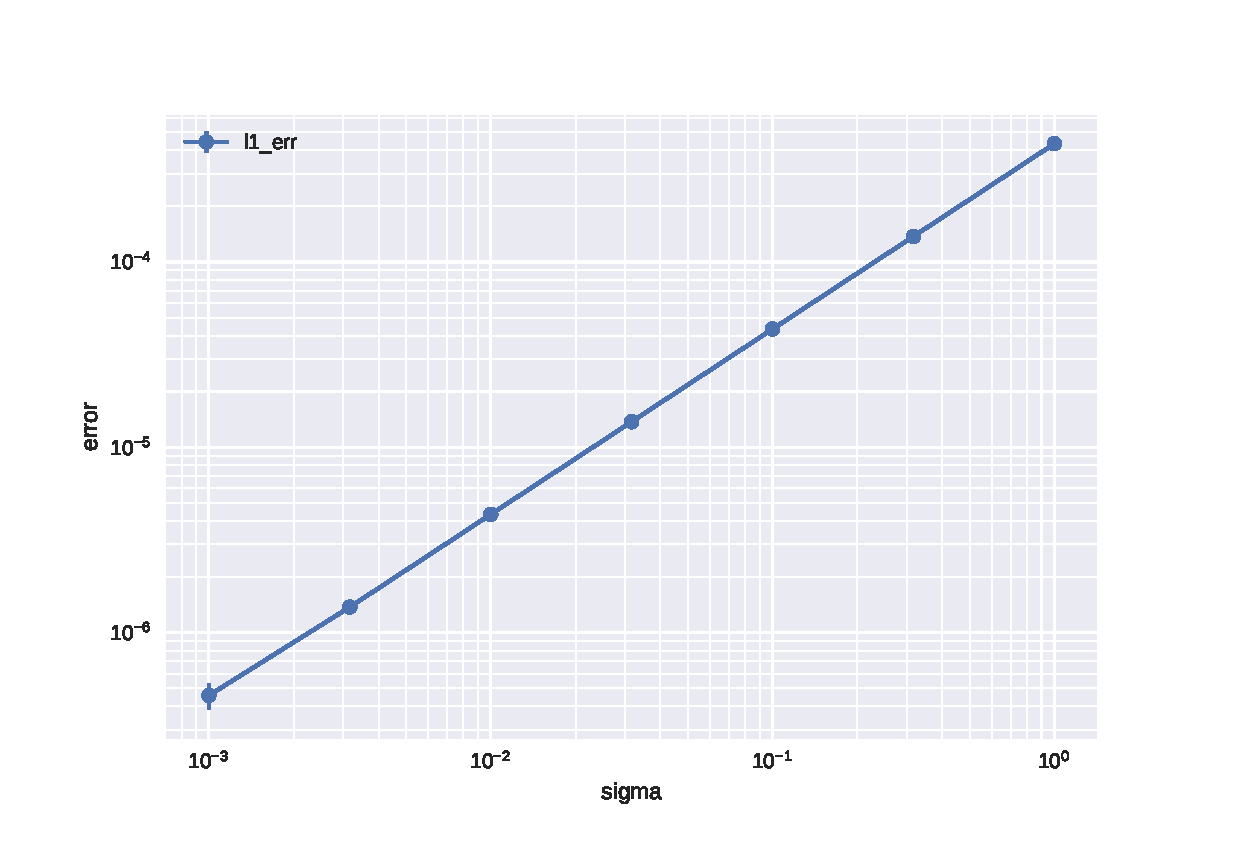
\includegraphics[scale=0.6]{./graph/noise}
\caption{Loglog plot of mean $L_1$ error versus $\sigma$. The mean $L_1$ error grows roughly linearly with $\sigma$. Errorbars are very small. \label{fig:noise}}
\end{figure}

\subsection{Binning benchmarks}
It is satisfying to see how binning speeds up as we make various code optimizations.

\begin{center}
\begin{tabular}{|c|c|c|}
\hline
Version & Running time/ns & Remarks \\
\hline
BinInTimeV0 & 51313717 & Reference implementation \\
BinInTimeV1 & 33825153 & Exploit symmetry \\
BinInTimeV2 & 15464899 & Chebyshev approximation \\
BinInTimeV3 & 15498434 & Boost.SIMD \\
BinInTimeV4 & 13177513 & Work with double instead of complex arrays \\
BinInFreqV0 & 189515 & Reference implementation \\
BinInFreqV1 & 91742 & Exploit symmetry\\
\hline
\end{tabular}
\end{center}

\bibliographystyle{abbrv}
\bibliography{references}

\end{document}